\chapter{Introduction} \label{chap:intro}

The process of finding similar and related concepts is one of the most characteristic activities of human nature and, specifically, of scientific research. Indeed, the categorisation of known concepts (\ie the proper distribution of the concepts in manageable categories, where each category contains only concepts that are similar to each other) introduces an abstraction layer over the reality that enables a more focussed reasoning over experimental results and empirical observations. The importance of categorisation is tightly coupled with the amount of concepts that one must deal with: as the amount of collective human knowledge increases, so does the needs for good categorisation that abstracts away the less useful details of reality, thereby increasing its manageability.

Therefore, similarity and relatedness measures are, without a doubt, necessary assets for the advancement of science. As we will see in this document, I argue that \emph{semantic} measures are, in fact, one of the most useful ways to achieve similarity and relatedness values for today's scientific resources, which are now sufficiently ripe for use in research, with particularly applicable results in the context of biomedical informatics.

The findings of this thesis focus primarily in the biomedical domain, given that the level of commitment in the biomedical informatics community to develop automatic systems to help their research (and ultimately contribute to the medical practice) is extremely high. For this reason, the whole document is written with a biomedical point of view. However, it is important to notice that the results that I will describe later and the contributions that stem from the work that I carried out can be generalised into other areas of research with minimal effort.


\section{Motivation} \label{sec:intro/motivation}

It is an undeniable and undisputed fact of scientific research that the amount of knowledge and data published each year is increasing at an exponential pace~\citep{Larsen2010}. This behaviour is true not only across areas of research but also across types of publication: it can be observed in the number of academic papers as well as in the sizes of databases, with staggering examples in protein databases \citep[\eg][]{Uniprot2010} or chemical databases~\citep{Williams2008}. Even clinical information can be collected (subject to ethic guidelines, given the need for confidentiality in such records) and used in research, a practice called translational medicine~\citep{Nalichowski2006,Wehling2008}. \figref{fig:medline-growth} illustrates this facet of scientific discovery by plotting the amount of articles contained in MEDLINE (a bibliographic database for the life sciences) against time, which shows an approximately exponential trend. The same behaviour can be observed in other databases of biomedical information, such as the one in \figref{fig:pdb-growth}.

\begin{figure}
    \centering
    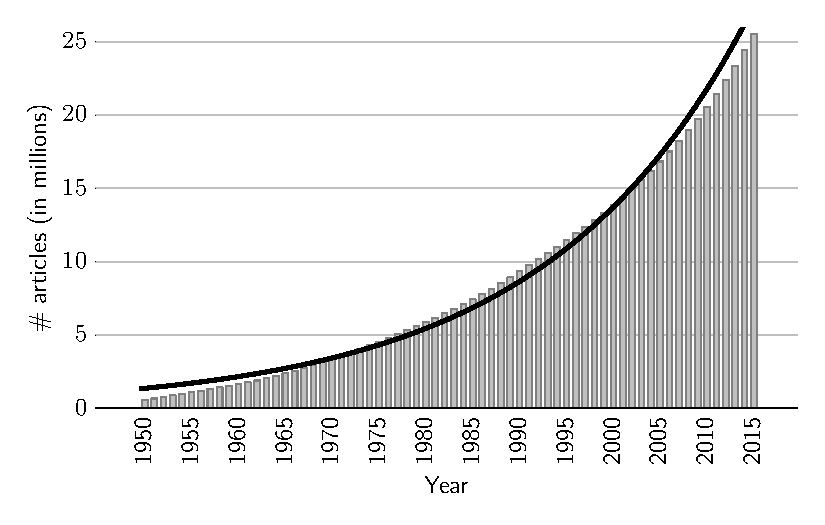
\includegraphics[width=0.8\textwidth]{images/medline-stats.pdf}
    \caption[Yearly size of MEDLINE from 1950 to~2015]{This plot shows that the number of bibliographic entries in MEDLINE has increased exponentially. The bars represent the cumulative number of articles indexed in this database each year, while the bold line is an exponential fit to the data. This rate of growth corresponds, on average, to a doubling in the amount of articles every $15.0$~years. Data retrieved from an actual search for publications between 1950 and~2015, in \url{http://www.ncbi.nlm.nih.gov/pubmed}. This image is meant as an illustration only, as there are many scientific results that are not published in MEDLINE-indexed journals.}
    \label{fig:medline-growth}
\end{figure}

\begin{figure}
    \centering
    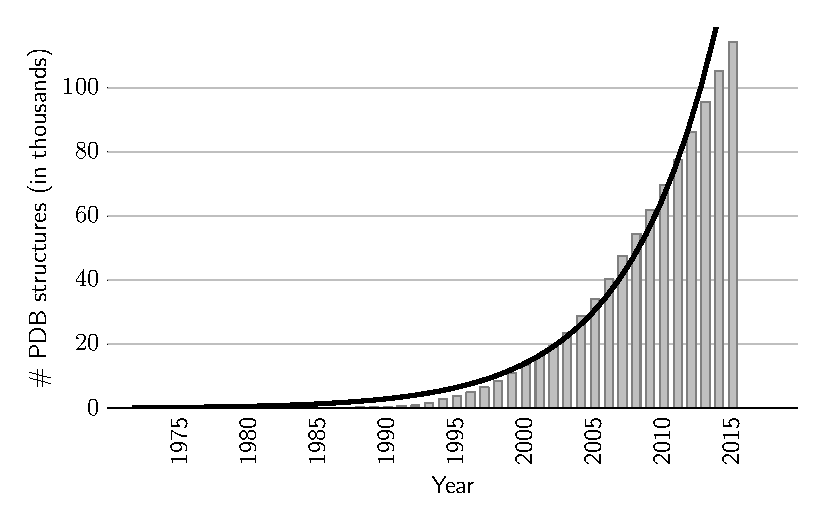
\includegraphics[width=0.8\textwidth]{images/pdb-stats.pdf}
    \caption[Number of $3$-dimensional protein structures in PDB from 1975 to~2015]{This plot shows that the number of protein structures stored in the Protein Data Bank has increased almost exponentially since the database has been created. The bars represent the total number of structures in this database, while the bold line is an exponential fit to the data. This rate of growth corresponds, on average, to a doubling in the size of the database every $4.5$~years. Data from \url{http://www.rcsb.org/pdb/statistics/contentGrowthChart.do?content=total}.}
    \label{fig:pdb-growth}
\end{figure}

   
With this exponential increase, two major problems have arisen. First, it has become impossible for researchers to fully read and interpret all the new information that becomes available each day. Second, and more important in scientific research, data published by different authors is often released in different formats, with different assumptions on what the meaning of each particular datum is. This makes it difficult, and in some cases impossible, to properly integrate all this information under a central knowledge repository without a lot of effort on the part of the data owners.

Surprisingly, these two problems are related, and solving one will help solve the other. Specifically, the impracticality of manually reading papers has created the need to develop automatic systems able to read textual documents, to appropriately parse and interpret them, and finally to draw conclusions based on them (for example by generating an automatic summary). To allow such a system to function, it must be able to understand the \emph{meaning} underlying the concepts referred to in the text, which, for example, includes understanding that the heart is responsible for pumping blood, that muscles are attached to bones through tendons, or that infections can cause fever. This, in turn, requires that knowledge be encoded in a machine-readable format, which must be precise, formal, and comprehensive, enabling computers to perform reasoning. Only that allows a computer to interpret text. On the other hand, knowledge that is described in such a format, using standard representations that everyone agrees with, can also be used by computers and, ultimately, be regarded as interoperable. This solves the second issue: if an automatic system is able to parse data from multiple sources in a logical format, it can use them uniformly as if they had the same provenance.

There are, today, many organisations dedicated to the production of formal standards for knowledge representation as well as \emph{reference knowledge artefacts} (called ontologies throughout this document), predominantly in the biomedical informatics community. For example, the Gene Ontology (\ontology{GO}), first published in 2000~\citep{Ashburner2000}, is an attempt to ``address the need for consistent descriptions of gene products in different databases''~\citep{GOIntroduction}. With the maturation of the standards for knowledge representation and the semantic web (see \secref{sec:concepts/knowledge-representation,sec:concepts/ontologies,sec:concepts/semantic-web} for a summary of the importance of these concepts to the field of biomedical informatics), \ontology{GO} has grown into a mature digital artefact that represents properties of proteins such as molecular function and cellular localization.

To explore the wealth of information that is stored in biomedical data, it is vital that ontology developers and users be provided with tools that can properly manage and handle the data; one ubiquitous requirement in science is the ability to estimate the degree of similarity or relatedness between the various ontology concepts~\citep{Vision2011} and, by extension, between multidisciplinary entities. For instance, similarity between proteins is often associated with one or more functions being shared among them~\citep{Altschul1990}; in chemistry, similarity of molecular structure correlates with similar biological role~\citep{Hansch1964,Klebe1994}; in medicine, a high degree of similarity between two clinical cases is a strong argument towards a similar diagnosis~\citep{Swender1974}.

One of the technologies enabled by the use of ontologies is indeed the calculation of similarity between the concepts they represent, a technique known as ``semantic similarity''~\citep{Resnik1995,Lord2003,Pesquita2009}. This technique can be used to compare concepts within one ontology as well as entities annotated with those concepts. For example, proteins annotated with \ontology{GO} functions can be compared based on the semantic similarity of those functions. While traditional automatic systems compared proteins by their sequence, using methods such as BLAST~\citep{Altschul1997}, semantic annotations provide a mechanism to compare proteins by their functions~\citep{Lord2003}. Advantages of this include the fact that some proteins that are known to have similar functions have different sequences, or vice-versa. Thus, semantic similarity can explicitly explore information about entities (in this case proteins) to more accurately compare them.

Semantic similarity has been applied to various domains:
\begin{itemize}
    \item between proteins annotated with \ontology{GO} concepts describing their molecular functions~\citep{Lord2003,Lei2006};
    \item between metabolic pathways annotated with their enzymes~\citep{Clemente2005} or chemical compounds~\citep{Grego2010}; and
    \item between diseases annotated with biological processes~\citep{Schlicker2010}.
\end{itemize}
Real world problems whose solution incorporates semantic similarity include the prediction of
\begin{paralist}
    \item the probability of a certain disease given a set of symptoms~\citep{Kohler2009},
    \item the cellular localization of proteins given their annotations~\citep{Lei2006},
    \item the function of proteins~\citep{Pesquita2008}, and
    \item the chemical properties of small metabolites~\citep{Ferreira2010}.
\end{paralist}

One of the remaining issues in this area is related to the fact that ontologies are often developed with a single domain of reality in mind. \ontology{GO} represents knowledge associated with proteins, \ontology{CHEBI} (Chemical Entities of Biological Interest) represents knowledge associated with biologically relevant chemical substances~\citep{Degtyarenko2008a}, \ontology{FMA} (Foundational Model of Anatomy) represents human anatomy~\citep{Rosse2003}, \etc. But knowledge is multidisciplinary, with some concepts from one domain being often intertwined with concepts from another domain. This is particularly true in the biomedical field, which is so vast that it is partitioned in several distinct but related disciplines. Clinical cases, for example, may include information on the symptoms, blood screen results, and drugs the patient is currently taking; even less obvious concepts, such as the previously visited places and the economical conditions of the patient can prove useful in tracing a diagnostic. Models of metabolic pathways refer to the reactions, the enzymes, the chemical metabolites the cellular components involved in the pathway, \etc. When accuracy is necessary (and it frequently is in the biomedical domain), multidisciplinarity naturally arises.

While single-ontology semantic similarity has been extensively studied in the last two decades, current algorithms are unable to adequately compare multidisciplinary entities. To handle multidisciplinarity, I propose that it is possible to harness the advantages of the existing single-ontology measures to allow their use in this context, by \emph{lifting} them from the single-ontology constraints. For this purpose, I study the following two approaches:
\begin{enumerate}
    \item Use single-ontology measures to compare concepts from the same domain in the two entities with single-ontology measures (\ie compare the chemical reactions of one entity with the chemical reactions of the other entity, then cellular components with cellular components, symptoms with symptoms, \etc.)\ and then combine the various results in a single value by means of an aggregating function such as the average. I call this the \emph{aggregative} approach.
    \item Use the inherent expressiveness of ontologies to integrate all knowledge in a single multidisciplinary knowledge base. Instead of calculating a value for each domain, this approach exploits the inter-domain links that exist between the ontologies to calculate multi-domain similarity and relatedness. For example, the relationship between skin and rash can be used to link together an ontology of anatomy and one of symptoms. I call this the \emph{integrative} approach.
\end{enumerate}


\section{Objective} \label{sec:intro/objective}

The theoretical objective of my PhD was to prove the following thesis:

\begin{quote}
Multi-domain semantic similarity measures can be constructed by lifting single-ontology measures according to the two approaches defined above (the aggregative and integrative approach), thus enabling semantic similarity on multidisciplinary entities.
\end{quote}
This statement is the driving force behind all the research efforts related to my work. In particular, I expect
\begin{paralist}
    \item that the comparison of multidisciplinary entities will be more effective when using a multi-domain measure rather than a single-ontology measure applied only to one domain, and
    \item that the integrative approach will generally be more effective than the aggregative approach, as it has access to more information.
\end{paralist}

\emph{Effectiveness} is an abstract concept that can have several interpretations depending on the context in which it is applied. In a medical context, a measure is effective if it can, for example, predict a disease from the clinical notes associated with a patient; in pharmacology, a measure is effective if it can be used to diminish the costs of drug tests by pre-emptively filtering potential drugs, thereby reducing the number of necessary trials. The proposed hypothesis, however, is orthogonal to the measure of effectiveness that one uses: irrespective of the way effectiveness is calculated, multi-domain measures perform well.

% As far as I was able to ascertain, no previous work has been published that explores the idea of multi-domain semantic similarity (more information on current methodologies in this area will be discussed in \chpref{chap:sota}). As such, evaluating the developed work will be a non-trivial task and as such the assessment of the \emph{effectiveness} of my similarity measures will not be as comprehensive as could be desired. However, there has been a recent \emph{hype} in the development of single-domain semantic similarity measures \citep[\eg][]{Lord2003,Pesquita2008,Kohler2009}, and as such the utility factor of multi-domain similarity measures (their effectiveness) can be evaluated through a direct comparison of the two approaches defined in the motivation. Given the nature of biomedical ontologies, specifically the dependency that exists between them, I was able to develop an integrated platform of similarity to better reflect the true similarity of biomedical concepts.

The practical and more fundamental objective of this thesis is, therefore, the creation of both
\begin{paralist}
    \item a semantic similarity framework that is able to deal with multidisciplinary entities, and
    \item semantic similarity measures that quantify these entities in a way that reflects their actual meaning.
\end{paralist}
For the first part, I will develop a system that is able to use existing single-ontology measures and lift them to multi-domain measures. For the second part, the focus will fall on finding use cases where multi-domain semantic similarity is needed, such as the detection of similar biochemical pathways or similar epidemiological resources. These datasets will be used to evaluate the effectiveness of multi-domain measures.

% \margin{This paragraph is weird!}
% Since there are ontologies that contain concepts for diseases (\eg the Human Disease Ontology), it could be argued that a single-ontology similarity measure on that ontology should suffice when comparing diseases. However, to correctly describe a disease, more information should be used. For instance, information such as the fact that some people with the flu exhibit fever symptoms does not fit into an ontology, since it is non-universal (not everyone with fever has the flu and not everyone with the flu displays fever symptoms). Treatments can be useful when comparing diseases, but the relation between treatment and disease is also non-universal. Furthermore, other biomedical entities, such as clinical cases, do not belong into ontologies, and are better described with explicit links to concepts. In these cases, multi-domain similarity measures are the only way to fully explore the wealth of information contained in these descriptions.


\section{Methodology} \label{sec:intro/methodology}

To achieve the main objective of this thesis, I had to fulfil five separate tasks.

% \point{Test preliminary single-domain measures}
% As a preliminary work, I have explored current techniques for \emph{single-domain} semantic similarity measures. To this effect, I continued my previous work on the Chemical Entities of Biological Interest (\ontology{CHEBI})~\citep{Ferreira2010}, using semantic similarity and machine-learning approaches to predict chemical compound functions; assisted in the development of semantic similarity for Geo-Net-PT~\citep{Batista2012}, an ontology of geospatial locations in Portugal; and devised a semantic \emph{relatedness} measure for the Foundational Model of Anatomy (\ontology{FMA})~\citep{Ferreira2011}.

\point{Study how validation is done in the field of semantic similarity}
Biomedical research in this field has been generating innovative and useful measures of similarity since~2003 and applying them to several distinct problems; however, validation is still being done in a relatively \emph{ad hoc} way, where each proposed measure is validated with a different method without much relation to previous ones. While some steps have been followed to mitigate this problem, a true systematization of validation strategies is still lacking, and as such one of the tasks of my work will be to determine to what extent this problem can be alleviated.

\point{Enhance current similarity and relatedness measures}
With the recent advance in the research of knowledge representation, ontologies are becoming increasingly richer and more expressive, and tools are being developed to handle this expressiveness. However, semantic similarity is not following this trend. For example, most algorithms are agnostic to the ideas of formal axioms, and as such are unable to use facts like the ones expressed with disjoint axioms (\ie there is no thing that is both a \term{Square} and a \term{Circle}) or other logic axioms. I believe that exploring in more detail the formal logic aspect of ontologies will yield measures of similarity that better reflect the structure of the ontology and the relationships between its concepts.

% The application of algorithms of ontology alignment will also prove invaluable to this thesis, since they find links between two ontologies, which enables the use of the integrative approach to multi-domain semantic similarity. As explained earlier, multi-domain measures need the integration of the several ontologies used, and this is only possible if there is a set of known facts between these concepts (\eg the previosuly mentioned relation between \term{Skin} and \term{Rash}).

% Another point of interest in this task is the exploration of machine-learning for the selection of attributes that better represent the concepts being compared. For example, a semantic similarity measure between two epidemiological resources may be dependent on the location of surge being studied, or on the economic conditions of that place, but in the domain of general diseases, the location may not be as relevant. In order to study the effect of all the information involved in the description of the objects being compared, there has to be a notion of how important these attributes are, which can be estimated with machine-learning approaches. This may be a critical step for the aggregative approach, since the exact features used must be carefully selected to yield a reasonable and practical measure.

% Additionally, the notion of \emph{information content} (see \secref{sec:concepts/ssm,sec:sota/node}) has been proved useful in single-domain similarity measures. This concept will probably play a major role in the measures of similarity, since it quantifies the specificity of ontology concepts. Therefore, the correct exploration of a multi-domain information content measure will be subject of study as well.

\point{Collect multidisciplinary datasets}
To test the measures of similarity and relatedness developed in this thesis, it will be necessary to collect multidisciplinary data annotated with concepts from various ontologies, which will allow the use of the aggregative and integrative approaches. Another important aspect of this task is the possibility to use the data collected and the help of experts to create gold-standards that can be used to validate the measures of similarity.

\point{Validate the multi-domain measures}
This task will finalise the proof of the proposed thesis by finding evidence that supports it. Validation of multi-domain semantic similarity measures can be done in several ways. For example, by comparing the automatically assigned similarity values with the ones assigned by experts in the gold-standards created in the previous task, or by using it in classification problems and quantifying the difference in performance between the single-ontology measures and the multi-domain approaches.

\point{Develop semantic similarity software}
Given the increasing number of ontologies, the amount of multidisciplinary data being published, and the growing standardization efforts in knowledge representation, it is more important than ever to develop the right tools to enable semantic similarity calculations in a reproducible way. As part of my contribution to this field, I will develop extensible software that will, on the one hand, allow developers to implement their semantic similarity measures under a common framework, and, on the other, provide users of semantic similarity (\eg online data repositories) a way to quickly calculate similarity between concepts or between annotated entities. This technical task will assist the previous task by allowing quick calculation of semantic similarity.


\section{Contributions} \label{sec:intro/contributions}

The contributions of this work can be summarised in terms of major and minor contributions. The five main contributions are aligned to the points delineated above:
\begin{enumerate}
    \item a hierarchy of validation strategies that can be used to classify research in semantic similarity according to the way the measures have been validated;
    \item an implementation of a single-ontology semantic relatedness measure, which can be generalised to the multi-domain context~\citep{Ferreira2011}, and of a single-ontology semantic similarity measure that can deal with disjointness axioms~\citep{Ferreira2013};
    \item the compilation of three multidisciplinary datasets, in the areas of epidemiology, metabolic pathways, and biochemical models, annotated with ontology concepts, onto which the multi-domain measures of similarity and relatedness operate;
    \item a validation of the two multi-domain approaches, by testing them on the multidisciplinary datasets and verifying that they outperform single-ontology measures; and
    \item the development of \owlsql\ and \mossy, two programs that work in tandem to provide easy semantic similarity calculations and which, in fact, already provide the implementations of the two multi-domain approaches.
\end{enumerate}

In the course of my work, I have additionally contributed to the epidemiology and geographical domains. The first of these minor contributions was the creation of a network of ontologies that are relevant in the domain of epidemiology and allow the formal categorization and annotation of epidemiological resources with ontology concepts, giving them semantic information that can be analysed by techniques like semantic similarity~\citep{Ferreira2012}. I have also contributed to an alignment between a geographical ontology of the Portuguese territory (Geo-Net-PT) and another ontology encoding the geo-political divisions of the world~\citep{Ferreira2010a}. Furthermore, I used semantic similarity in this domain to create a disambiguation algorithm that maps geographical names in text to the correct concept in Geo-Net-PT~\citep{Batista2012}. Finally, I have helped develop a text-mining system for the chemical domain that uses semantic similarity to validate its results~\citep{Lamurias2015}.

A brief summary of my main contributions can be examined in \secref{sec:conclusions/contributions}, and is complemented in \appref{app:auxiliary-projects} with a small description of my minor contributions.


\section{A word on terminology and notation} \label{sec:intro/notation}

Throughout this document, I will make numerous references to terms that are essential to describe the field of semantic similarity. \chpref{chap:concepts} will explain most of these terms, both to introduce the reader to these notions and to standardise the terminology, thus allowing a more thorough understanding of the document. To further assist the reader, the following typographical notation is used:
\begin{itemize}
    \item a blackboard font is used for ontology acronyms (\eg \ontology{GO}, \ontology{CHEBI});
    \item a \term{sans-serif font} is used to refer to concepts, always starting with a capital letter (\eg \term{Head}, \term{ATP binding}); and
    \item \prop{italic shape} is used for relationships between concepts, always in lower case and with spaces translated to hyphens (\eg \prop{part-of}).
\end{itemize}


\section{Structure of this document} \label{sec:intro/structure}

This document is organised in four parts.

The first part deals with the contextualization of the problem underlying the proposed hypothesis. Chapter~\ref{chap:concepts} defines and explains the basic notions needed to understand the problem itself, and Chapter~\ref{chap:sota} surveys the \emph{state of the art} with respect to how semantic similarity has been conducted both in the single-ontology and multiple-ontology contexts.

The second part accounts for my contributions. It contains five chapters, in parallel to the five points delineated in the methodology. Namely, Chapter~\ref{chap:validation} describes how the hierarchy of validation approaches was constructed, Chapter~\ref{chap:enhancements} outlines the enhancements that I propose for improving single-ontology semantic similarity, Chapter~\ref{chap:data} presents three multidisciplinary datasets collected to test the hypothesis, and Chapter~\ref{chap:multidomain} formally defines the two multi-domain semantic similarity approaches and demonstrates their performance on the multidisciplinary datasets, thus establishing the validity of the proposed hypothesis. Chapter~\ref{chap:technical}, although an indispensable part of the document, describes not direct scientific research but rather the technical aspects necessary for the execution of this methodology, by characterising the software that I developed to perform semantic similarity calculations.

The third part is composed of Chapter~\ref{chap:conclusions}, which enumerates some conclusions, limitations of my contributions and potential future work.

The last part deals with the appendixes, where I explain some of the details of the work in more detail than was possible in the main document, including Appendix~\ref{app:ontologies}, which contains a list of relevant ontologies used throughout my work and Appendix~\ref{app:auxiliary-projects}, which describes three research efforts where I participated that are related (if only tangentially) to my work. Finally, the document ends with a list of references.

